% =====================================================================
%  V2V-Project -- Study Pack
%  Section S7 : The Flask Monitoring Dashboard
%  Source files studied: dashboard/app.py , dashboard/templates/dashboard.html
%  Standalone document -- compile with:  pdflatex 07-monitoring-dashboard.tex
% =====================================================================
\documentclass[11pt,a4paper]{article}

\usepackage[utf8]{inputenc}
\usepackage[T1]{fontenc}
\usepackage{lmodern}

\usepackage[a4paper,margin=2.4cm]{geometry}
\usepackage{enumitem}
\setlist{topsep=2pt,itemsep=2pt}

\usepackage{amsmath}
\usepackage{amssymb}
\usepackage{booktabs}
\usepackage{graphicx}
\usepackage{xcolor}
\usepackage{listings}
\usepackage{tikz}
\usetikzlibrary{arrows.meta,positioning,shapes.geometric,calc,fit,backgrounds}
\usepackage[colorlinks=true,linkcolor=blue,urlcolor=blue,citecolor=blue]{hyperref}

\definecolor{codebg}{rgb}{0.97,0.97,0.94}
\definecolor{codegreen}{rgb}{0.00,0.50,0.00}
\definecolor{codegray}{rgb}{0.50,0.50,0.50}
\definecolor{keyblue}{rgb}{0.00,0.20,0.70}
\definecolor{boxblue}{rgb}{0.88,0.93,1.00}
\definecolor{boxyellow}{rgb}{1.00,0.97,0.85}

\lstdefinestyle{py}{
  language=Python,
  backgroundcolor=\color{codebg},
  basicstyle=\ttfamily\footnotesize,
  keywordstyle=\color{keyblue}\bfseries,
  stringstyle=\color{codegreen},
  commentstyle=\color{codegray}\itshape,
  numberstyle=\tiny\color{codegray},
  numbers=left,
  numbersep=8pt,
  showstringspaces=false,
  breaklines=true,
  breakatwhitespace=false,
  frame=single,
  rulecolor=\color{codegray},
  tabsize=4,
  captionpos=b,
}
\lstdefinestyle{web}{
  backgroundcolor=\color{codebg},
  basicstyle=\ttfamily\footnotesize,
  numberstyle=\tiny\color{codegray},
  numbers=left,
  numbersep=8pt,
  showstringspaces=false,
  breaklines=true,
  frame=single,
  rulecolor=\color{codegray},
  tabsize=2,
  captionpos=b,
}
\lstdefinestyle{term}{
  backgroundcolor=\color{codebg},
  basicstyle=\ttfamily\footnotesize,
  breaklines=true,
  frame=single,
  rulecolor=\color{codegray},
  numbers=none,
  captionpos=b,
}

\title{\textbf{V2V-Project Study Pack}\\[4pt]
       \large Section S7 --- The Flask Monitoring Dashboard}
\author{Information Security Project --- Beginner Study Notes}
\date{Source files: \texttt{dashboard/app.py}, \texttt{dashboard/templates/dashboard.html}}

\begin{document}
\maketitle
\tableofcontents
\newpage

% =====================================================================
\section{Title and ``What You'll Learn''}
% =====================================================================

\subsection*{Section Title}
\textbf{S7 --- The Monitoring Dashboard: a small web page that lets a human
\emph{watch} the secure V2V system work in real time.}

\subsection*{Plain-English Summary (read this first)}
The security work is done by Sections~S2--S6. Section~S7 adds \emph{eyes}: a web
page, served by a tiny \textbf{Flask} web application, that shows --- live --- a
vehicle's certificate status, whether it has authenticated, how many messages it
has sent and received, and any security alerts. The browser asks the server
``what is happening now?'' every three seconds and re-draws the page. It is
crucial to understand that the dashboard is a \emph{window}, not a \emph{lock}:
it \emph{observes} security, it does not \emph{enforce} it.

\subsection*{Learning Outcomes}
After studying this section you will be able to:
\begin{itemize}
  \item Explain what \textbf{Flask}, a \textbf{web server} and an
        \textbf{HTTP route} are.
  \item Explain a \textbf{REST API} and the difference between \textbf{GET} and
        \textbf{POST}.
  \item Explain \textbf{JSON} as the language between browser and server.
  \item Explain \textbf{polling} and why the page refreshes every 3 seconds.
  \item Explain what \textbf{CORS} is and why it appears here.
  \item Walk through all four routes in \texttt{app.py} and the JavaScript in
        \texttt{dashboard.html}.
  \item Explain why the dashboard is \emph{observability}, not a security control.
\end{itemize}

% =====================================================================
\section{Where This Fits}
% =====================================================================

S7 sits \emph{beside} the pipeline, not inside it. The three security stages
(Identity, Authentication, Secure Messaging) run inside the vehicle node of S6.
S7 attaches a viewing window to that running node: \texttt{app.py} reads the
node's state through the \texttt{get\_state()} method (introduced in S6) and
serves it to a browser. If you removed S7 entirely, the cars would still
communicate just as securely --- you simply would not be able to \emph{see} it.

\begin{center}
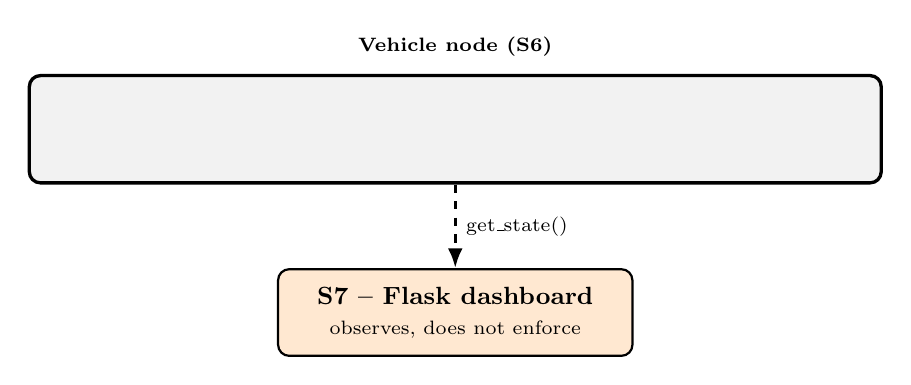
\begin{tikzpicture}[font=\small,node distance=8mm and 12mm,
   st/.style={draw,rounded corners,minimum width=2.7cm,minimum height=1.1cm,
              align=center,thick}]
  \node[st,fill=boxblue]   (id)   {Identity\\\scriptsize S2};
  \node[st,fill=green!12,right=of id]   (au) {Authentication\\\scriptsize S4};
  \node[st,fill=boxyellow,right=of au] (ms) {Messaging\\\scriptsize S5};
  \node[draw,very thick,rounded corners,fill=gray!10,fit=(id)(au)(ms)] (vn) {};
  \node[above=1mm of vn,font=\scriptsize\bfseries] {Vehicle node (S6)};
  \node[st,fill=orange!18,below=12mm of au,minimum width=4.5cm] (dash)
       {\textbf{S7 -- Flask dashboard}\\\scriptsize observes, does not enforce};
  \draw[-{Latex[length=2.5mm]},very thick,dashed] (vn) -- (dash)
       node[midway,right,font=\scriptsize]{get\_state()};
\end{tikzpicture}
\end{center}

% =====================================================================
\section{The Theory You Must Study}
% =====================================================================

\subsection{Web Server, Flask and HTTP}
\textbf{Plain definition.} A \textbf{web server} is a program that answers
requests from web browsers. \textbf{HTTP} (HyperText Transfer Protocol) is the
language of those requests and answers. \textbf{Flask} is a small, popular Python
library for building web servers.

\textbf{Real-life analogy.} A web server is an information desk. HTTP is the
fixed call-and-response format: a visitor asks a question (``request''), the desk
gives an answer (``response''). Flask is a starter kit for setting up that desk.

\textbf{Why it exists.} People want to \emph{see} the V2V system in an ordinary
web browser. A web server is what lets a browser ask for and receive a page.

\textbf{How it works here.} \texttt{app.py} calls \texttt{Flask(\_\_name\_\_)} to
create the server, then defines a few \emph{routes}. \texttt{vehicle\_node.py}
runs this Flask app in a background daemon thread.

\textbf{Security property it provides.} None --- the dashboard is a viewer.

\subsection{Routes / Endpoints}
\textbf{Plain definition.} A \textbf{route} (or \emph{endpoint}) is a specific
web address the server knows how to answer, paired with the code that produces
the answer.

\textbf{Real-life analogy.} The different windows at a post office: ``Stamps'',
``Parcels'', ``Complaints''. Each address goes to a specific window with specific
staff.

\textbf{Why it exists.} One server must answer several different questions ---
``give me the page'', ``give me the live data'', ``clear the alerts''. Routes
keep each question separate.

\textbf{How it works here.} The \texttt{@app.route("/...")} decorator above a
function says ``when a browser asks for this address, run this function''.
\texttt{app.py} defines four routes.

\textbf{Security property it provides.} None directly.

\subsection{REST API, GET and POST}
\textbf{Plain definition.} An \textbf{API} (Application Programming Interface) is
a way for one program to ask another for data or actions. A \textbf{REST API}
over HTTP uses different \emph{methods}: \textbf{GET} \emph{reads} data (and
changes nothing); \textbf{POST} \emph{sends} data or \emph{triggers a change}.

\textbf{Real-life analogy.} GET is \emph{looking at} the noticeboard. POST is
\emph{pinning a new note} to it. Looking changes nothing; pinning does.

\textbf{Why it exists.} The browser needs two kinds of interaction: fetch the
latest state (read) and clear the alerts (change). Using GET for reads and POST
for changes keeps the design clean and predictable.

\textbf{How it works here.} \texttt{/api/state} and \texttt{/api/alerts} are GET
routes (read-only). \texttt{/api/clear-alerts} is a POST route
(\texttt{methods=["POST"]}) because it changes something --- it empties the alert
list.

\textbf{Security property it provides.} None directly, though using GET only for
safe reads is good hygiene.

\subsection{JSON --- the Browser/Server Language}
\textbf{Plain definition.} \textbf{JSON} (JavaScript Object Notation) is a simple
text format for structured data --- names paired with values, in braces.

\textbf{Real-life analogy.} A filled-in form with labelled boxes:
\texttt{vehicle\_id: vehicle-a, total\_sent: 42}.

\textbf{Why it exists.} The Python server and the JavaScript in the browser are
different languages, but both understand JSON, so it is the neutral format they
exchange.

\textbf{How it works here.} Flask's \texttt{jsonify(...)} turns a Python
dictionary into a JSON response. In the browser, \texttt{await r.json()} turns
that JSON text back into a JavaScript object the page can read.

\textbf{Security property it provides.} None --- it is a data format.

\subsection{Polling}
\textbf{Plain definition.} \textbf{Polling} means the browser repeatedly asks
``anything new?'' on a timer, rather than the server pushing updates.

\textbf{Real-life analogy.} Refreshing your email inbox every few minutes instead
of waiting for a notification.

\textbf{Why it exists.} It is the \emph{simplest} way to keep a page up to date.
The dashboard does not need split-second freshness, so a humble timer is enough
--- no need for more complex ``push'' technology.

\textbf{How it works here.} The JavaScript line \texttt{setInterval(fetchState,
3000)} runs \texttt{fetchState} every 3000~milliseconds (3 seconds). Each call
fetches \texttt{/api/state} and redraws the page.

\textbf{Security property it provides.} None.

\subsection{CORS}
\textbf{Plain definition.} \textbf{CORS} (Cross-Origin Resource Sharing) is a
browser security rule that, by default, stops a page loaded from one web address
from reading data from a \emph{different} address. A server can relax this rule
with special response headers.

\textbf{Real-life analogy.} A building security rule: a visitor with a ``Floor~5''
pass cannot wander onto Floor~3. CORS headers are the management explicitly
saying ``actually, let this pass work on Floor~3 too''.

\textbf{Why it exists here.} Vehicle~A's dashboard runs on port~5001 and
Vehicle~B's on port~5002 --- the browser treats those as different ``origins''.
To let a page on one port read the API on another, the server must allow it.

\textbf{How it works here.} An \texttt{@app.after\_request} hook adds the header
\texttt{Access-Control-Allow-Origin: *}. The \texttt{*} means ``any origin may
read this API''.

\textbf{Security property it provides.} CORS is itself a security mechanism ---
but here it is \emph{loosened} to \texttt{*}. That is fine for a local classroom
demo, but in a real deployment an open \texttt{*} on an unauthenticated API would
be a weakness. (More on this in the Attack Relevance section.)

% =====================================================================
\section{Code Walkthrough}
% =====================================================================

\subsection{File: dashboard/app.py --- the Flask server}

\subsubsection*{create\_app() --- build the web application}
\textbf{Purpose:} create the Flask app, bind it to a running vehicle node, and
define the routes.
\begin{lstlisting}[style=py,caption={dashboard/app.py --- the whole Flask application.}]
def create_app(node) -> Flask:
    app = Flask(__name__,
                template_folder=str(Path(__file__).parent / "templates"))

    @app.after_request
    def _cors(response):
        response.headers["Access-Control-Allow-Origin"] = "*"
        response.headers["Access-Control-Allow-Methods"] = "GET, POST, OPTIONS"
        response.headers["Access-Control-Allow-Headers"] = "Content-Type"
        return response

    @app.route("/")
    def index():
        return render_template("dashboard.html")

    @app.route("/api/state")
    def api_state():
        return jsonify(node.get_state())

    @app.route("/api/alerts")
    def api_alerts():
        return jsonify({"alerts": node.logger.get_alerts()})

    @app.route("/api/clear-alerts", methods=["POST"])
    def api_clear_alerts():
        node.logger.clear_alerts()
        return jsonify({"status": "cleared"})

    return app
\end{lstlisting}
\textbf{Step by step:}
\begin{enumerate}
  \item \texttt{create\_app(node)} takes the running \texttt{VehicleNode} (from
        S6) so the dashboard has a live data source.
  \item \texttt{Flask(...)} creates the server; \texttt{template\_folder} tells
        it where the HTML page lives.
  \item The \texttt{\_cors} function, marked \texttt{@app.after\_request}, runs
        \emph{after every response} and adds the CORS headers (see the theory
        above).
  \item Route \texttt{"/"} --- the home page. \texttt{render\_template} loads and
        returns \texttt{dashboard.html}.
  \item Route \texttt{"/api/state"} --- a GET endpoint. It calls the node's
        \texttt{get\_state()} and \texttt{jsonify}s the dictionary. This is the
        endpoint the browser polls every 3 seconds.
  \item Route \texttt{"/api/alerts"} --- a GET endpoint returning just the alert
        list.
  \item Route \texttt{"/api/clear-alerts"} --- a POST endpoint
        (\texttt{methods=["POST"]}) because it \emph{changes} state: it calls
        \texttt{clear\_alerts()} and confirms with \texttt{\{"status":
        "cleared"\}}.
\end{enumerate}
\textbf{Arguments / return:} \texttt{create\_app} takes \texttt{node} and returns
the Flask \texttt{app}; \texttt{vehicle\_node.py} then runs it in a thread.
\textbf{Theory link:} routes, REST (GET vs POST), JSON, CORS.
\emph{Analogy:} \texttt{app.py} is the information desk; each route is one
window.

\subsubsection*{The data source: node.get\_state()}
\texttt{app.py} itself produces no data --- it is a thin layer. The real content
comes from the vehicle node's \texttt{get\_state()} method (studied in S6), which
returns a dictionary of: \texttt{vehicle\_id}, certificate status and expiry,
authentication status, peer id, whether a session is active, the recent messages,
the alert list, and the statistics counters. \texttt{/api/state} just wraps that
dictionary in JSON.

\subsection{File: dashboard.html --- the page and its JavaScript}

\subsubsection*{The page structure (HTML)}
The HTML body has four visible regions:
\begin{enumerate}
  \item A \textbf{header} with the title.
  \item Three \textbf{status cards}: ``Certificate Status'', ``Authentication
        Status'' and ``Security Alerts'' (the last one has a \emph{Clear Alerts}
        button).
  \item A \textbf{stats row} of four boxes: Messages Sent, Messages Received,
        Attacks Blocked, Session Active.
  \item A \textbf{Recent Messages table} with one row per message and a tick/cross
        for each security property.
\end{enumerate}
Every value on the page starts as a placeholder (\texttt{--} or \texttt{LOADING})
and is filled in by JavaScript once the first data arrives.

\subsubsection*{The CSS (styling) --- one security-relevant detail}
Most of the CSS is cosmetic (a dark theme, rounded cards). One rule \emph{is}
worth noting --- the blinking-alert animation:
\begin{lstlisting}[style=web,caption={dashboard.html --- the alert-blink CSS (decorative comment dashes simplified).}]
/* -- Blinking alert card -- */
@keyframes blink-red {
  0%, 100% { border-color: #f85149; box-shadow: 0 0 15px rgba(248,81,73,0.4); }
  50%      { border-color: #30363d; box-shadow: none; }
}
.alert-active { animation: blink-red 1s infinite; }
\end{lstlisting}
When JavaScript adds the class \texttt{alert-active} to the alert card, this
animation makes it flash red once per second --- so a security alert is
impossible to miss on screen.

\subsubsection*{The JavaScript --- fetch, update, repeat}
\begin{lstlisting}[style=web,caption={dashboard.html --- the polling JavaScript (core parts).}]
async function fetchState() {
  try {
    const r = await fetch('/api/state');   // GET the live state
    const d = await r.json();              // parse JSON into an object
    update(d);                             // redraw the page
  } catch (e) { console.error('Fetch failed', e); }
}

function update(d) {
  // Certificate card
  const cb = document.getElementById('cert-badge');
  cb.textContent = d.cert_status;
  cb.className = 'badge ' + (d.cert_status === 'VALID' ? 'badge-green' : 'badge-red');
  // Alert card -- turn the card red and blinking if there are alerts
  const alerts = d.alerts || [];
  if (alerts.length > 0) {
    document.getElementById('alert-card').classList.add('alert-active');
  } else {
    document.getElementById('alert-card').classList.remove('alert-active');
  }
  // Stats: Attacks Blocked = tamper blocked + replay blocked
  const s = d.stats || {};
  document.getElementById('stat-blocked').textContent =
      (s.tamper_attempts_blocked || 0) + (s.replay_attempts_blocked || 0);
  // ... fill the message table row by row ...
}

async function clearAlerts() {
  await fetch('/api/clear-alerts', { method: 'POST' });   // POST
  fetchState();
}

setInterval(fetchState, 3000);   // poll every 3 seconds
fetchState();                    // and once immediately
\end{lstlisting}
\textbf{Step by step:}
\begin{enumerate}
  \item \texttt{fetchState} is \texttt{async} --- it sends a GET request to
        \texttt{/api/state}, \texttt{await}s the reply, and parses the JSON.
  \item \texttt{update(d)} takes that data object and writes it into the page:
        it sets the certificate badge text and colour, shows/clears the blinking
        alert state, fills the four stat boxes (note ``Attacks Blocked'' is the
        \emph{sum} of tamper and replay counters), and rebuilds the message
        table.
  \item \texttt{clearAlerts} sends a \texttt{POST} to \texttt{/api/clear-alerts}
        (this is the only state-changing call the page makes), then immediately
        refetches.
  \item \texttt{setInterval(fetchState, 3000)} repeats the fetch every 3 seconds;
        the bare \texttt{fetchState()} call runs once at page load so the user
        does not wait 3 seconds for the first data.
\end{enumerate}
\textbf{Theory link:} polling; GET for reads, POST for the change; JSON as the
shared format. \emph{Analogy:} a receptionist who phones the back office every 3
seconds and re-writes the whiteboard with the latest news.

% =====================================================================
\section{Hands-On / Practical}
% =====================================================================

\subsection{Open the dashboard}
Start a vehicle node as in Section~S6 (it launches the dashboard automatically),
then open a browser at the dashboard address printed in the log:
\begin{lstlisting}[style=term]
http://localhost:5001        (Vehicle A)
http://localhost:5002        (Vehicle B)
\end{lstlisting}

\noindent You can also confirm the API directly without a browser, using
PowerShell:
\begin{lstlisting}[style=term]
curl http://localhost:5001/api/state
\end{lstlisting}

\noindent\textbf{Expected output (sample of the \texttt{/api/state} JSON):}
\begin{lstlisting}[style=term]
{
  "vehicle_id": "vehicle-a",
  "cert_status": "VALID",
  "cert_cn": "vehicle-a",
  "cert_expiry": "2027-05-17",
  "auth_status": "AUTHENTICATED",
  "peer_id": "vehicle-b",
  "session_active": true,
  "recent_messages": [ ... ],
  "alerts": [],
  "stats": {"total_sent": 12, "total_received": 11,
            "tamper_attempts_blocked": 0, "replay_attempts_blocked": 0}
}
\end{lstlisting}

\subsection{What the dashboard shows}
\begin{itemize}
  \item \textbf{Certificate Status card} --- \texttt{VALID} (green) if the
        vehicle's certificate parsed correctly.
  \item \textbf{Authentication Status card} --- \texttt{AUTHENTICATED} (green)
        once the handshake has completed; shows the peer id.
  \item \textbf{Security Alerts card} --- \texttt{0 ALERTS} (green) normally; if
        an attack is blocked it turns red and \emph{blinks}.
  \item \textbf{Stats row} --- live counts of messages sent, received, attacks
        blocked, and whether a session is active.
  \item \textbf{Recent Messages table} --- the last 20 messages, each with
        green ticks for Auth / Encrypted / Integrity / Replay-protected.
\end{itemize}

\subsection{Illustration placeholder --- dashboard screenshot}
\begin{center}
\fbox{\parbox{0.85\textwidth}{\centering\vspace{1.2cm}
\textbf{[ ADD SCREENSHOT HERE ]}\\[4pt]
Run a vehicle node, open \texttt{http://localhost:5001} in a browser, take a
screenshot of the live dashboard, save it as \texttt{dashboard.png} in this
folder, and replace this box with:\\[4pt]
\texttt{\textbackslash includegraphics[width=0.85\textbackslash textwidth]\{dashboard.png\}}
\vspace{1.2cm}}}
\end{center}

\subsection{Try This Yourself (mini-experiment)}
With the two vehicle nodes running and the dashboard open, run an attack script
against the system (for example \texttt{python attacks\textbackslash
tamper\_attack.py}, Section~S8) --- or simply note what \emph{would} happen:
when a TAMPER or REPLAY alert is logged, the node's \texttt{get\_state()} returns
a non-empty \texttt{alerts} list.\\
\textbf{Predict before you run.} On the \emph{next} 3-second poll, the JavaScript
\texttt{update} function sees \texttt{alerts.length > 0}, adds the
\texttt{alert-active} class to the alert card, and the card starts blinking red;
the ``Attacks Blocked'' number ticks up. Now click \emph{Clear Alerts}: a POST is
sent, the alert list empties, and on the next poll the card goes calm green
again. As a second experiment, change \texttt{setInterval(fetchState, 3000)} to
\texttt{1000} --- predict the page now refreshes once per second instead of every
three.

% =====================================================================
\section{Attack Relevance}
% =====================================================================

\textbf{The dashboard defends against \emph{nothing}.} This is the single most
important point of S7, and an examiner will test it. The dashboard is
\textbf{observability}: it makes the work of the real defences \emph{visible to a
human}. It is the difference between a smoke alarm (a defence-adjacent alert) and
the sprinkler system (the actual defence).

\medskip
\noindent What the dashboard \emph{does} contribute:
\begin{itemize}
  \item It \textbf{surfaces} blocked attacks. When S5/S6 reject a tampered or
        replayed message, the alert is logged; the dashboard turns it into a
        blinking red card and an ``Attacks Blocked'' counter --- so a human
        immediately sees the system is under attack and is holding.
  \item It builds \textbf{confidence}: the green ticks per message let an
        observer confirm every BSM really was authenticated, encrypted,
        integrity-checked and replay-protected.
\end{itemize}

\medskip
\noindent\textbf{Honest weaknesses of the dashboard itself.} If an examiner asks
``could the dashboard be attacked?'', the honest answer is yes, in two ways, and
neither affects the V2V security itself:
\begin{enumerate}
  \item \textbf{The API is unauthenticated.} Anyone who can reach port~5001 can
        \texttt{GET /api/state} and read the vehicle's status, or
        \texttt{POST /api/clear-alerts} to wipe the alert history. There is no
        password on the dashboard.
  \item \textbf{CORS is wide open} (\texttt{Access-Control-Allow-Origin: *}), so
        any web page in the browser could read the API.
\end{enumerate}
For a local classroom demo this is acceptable and is a deliberate simplification.
In a real deployment the monitoring interface would need authentication and a
restricted CORS policy. Crucially, even if an attacker cleared the alert log,
they would \emph{not} weaken the cars' encryption, signatures or handshake ---
they would only blind the \emph{viewer}.

% =====================================================================
\section{Illustrations}
% =====================================================================

\subsection{Diagram 1 --- browser, Flask and the vehicle node}
\begin{center}
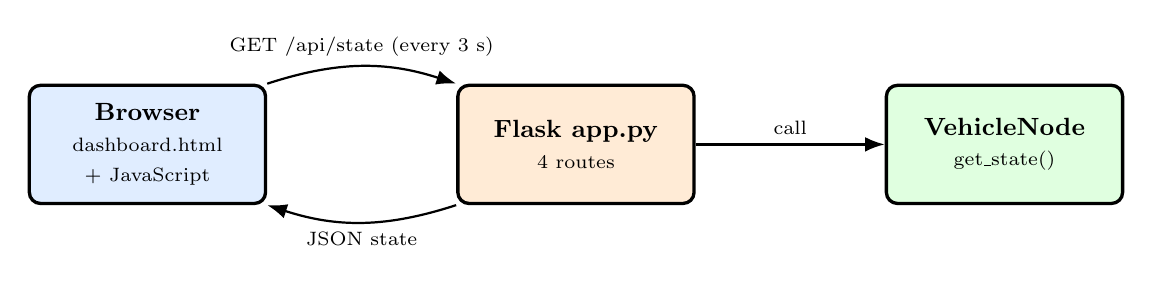
\begin{tikzpicture}[font=\small,node distance=14mm,
   b/.style={draw,very thick,rounded corners,minimum width=3.0cm,minimum height=1.5cm,
             align=center}]
  \node[b,fill=boxblue]  (br) {\textbf{Browser}\\\scriptsize dashboard.html\\\scriptsize + JavaScript};
  \node[b,fill=orange!16,right=24mm of br] (fl) {\textbf{Flask app.py}\\\scriptsize 4 routes};
  \node[b,fill=green!12,right=24mm of fl] (nd) {\textbf{VehicleNode}\\\scriptsize get\_state()};
  \draw[-{Latex[length=2.5mm]},thick] (br.north east) to[bend left=18]
       node[midway,above,font=\scriptsize]{GET /api/state (every 3 s)} (fl.north west);
  \draw[{Latex[length=2.5mm]}-,thick] (br.south east) to[bend right=18]
       node[midway,below,font=\scriptsize]{JSON state} (fl.south west);
  \draw[-{Latex[length=2.5mm]},thick] (fl) -- (nd)
       node[midway,above,font=\scriptsize]{call};
\end{tikzpicture}
\end{center}

\subsection{Diagram 2 --- the polling loop}
\begin{center}
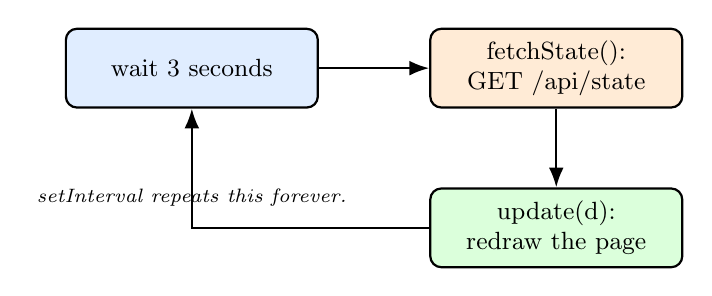
\begin{tikzpicture}[font=\small,node distance=9mm,
   s/.style={draw,thick,rounded corners,minimum width=3.2cm,minimum height=1.0cm,
             align=center}]
  \node[s,fill=boxblue] (wait) {wait 3 seconds};
  \node[s,fill=orange!16,right=14mm of wait] (fetch) {fetchState():\\GET /api/state};
  \node[s,fill=green!14,below=10mm of fetch] (upd) {update(d):\\redraw the page};
  \draw[-{Latex[length=2.5mm]},thick] (wait) -- (fetch);
  \draw[-{Latex[length=2.5mm]},thick] (fetch) -- (upd);
  \draw[-{Latex[length=2.5mm]},thick] (upd) -| (wait);
  \node[below=9mm of wait,font=\scriptsize\itshape] {setInterval repeats this forever.};
\end{tikzpicture}
\end{center}

% =====================================================================
\section{Presentation Pack}
% =====================================================================

\subsection{Slide Outline}

\textbf{Slide 1 --- What the Dashboard Is.}
\begin{itemize}
  \item A small web page that shows the V2V system live.
  \item Built with Flask (a Python web framework).
  \item Shows certificates, authentication, stats, alerts.
  \item It is a \emph{window}, not a \emph{lock}.
\end{itemize}

\textbf{Slide 2 --- How the Browser and Server Talk.}
\begin{itemize}
  \item Four routes: the page, state, alerts, clear-alerts.
  \item GET reads data; POST changes data.
  \item They exchange JSON --- the shared data format.
  \item CORS headers allow the cross-port setup.
\end{itemize}

\textbf{Slide 3 --- Polling: Always Up to Date.}
\begin{itemize}
  \item \texttt{setInterval(fetchState, 3000)} --- ask every 3 seconds.
  \item \texttt{fetchState} GETs \texttt{/api/state}, parses JSON.
  \item \texttt{update} redraws cards, stats and the message table.
  \item Simple timer; no complex push technology needed.
\end{itemize}

\textbf{Slide 4 --- Seeing an Attack.}
\begin{itemize}
  \item Blocked attacks become alerts in the node's logger.
  \item The alert card turns red and \emph{blinks}.
  \item ``Attacks Blocked'' = tamper blocked + replay blocked.
  \item \emph{Clear Alerts} button POSTs to reset the list.
\end{itemize}

\textbf{Slide 5 --- Observability, Not Enforcement.}
\begin{itemize}
  \item The dashboard defends nothing --- S2--S6 do that.
  \item It makes the defences visible and builds confidence.
  \item Honest weakness: the API has no password; CORS is open.
  \item Clearing alerts blinds the viewer --- it does not weaken the cars.
\end{itemize}

\subsection{Speaker Talking Points (about 30--60 seconds each)}

\textbf{Slide 1.} ``Sections two through six do the actual security work. Section
seven adds eyes. It is a small web page, served by a tiny Python web application
built with Flask, that shows the system working in real time --- the
certificate's status, whether the cars have authenticated, how many messages have
flowed, and any security alerts. The key idea, and I will keep repeating it, is
that this dashboard is a window, not a lock. It lets you watch the security; it
does not provide the security.''

\textbf{Slide 2.} ``The browser and the server talk over HTTP using four routes.
One route serves the HTML page itself. One returns the live state. One returns
just the alerts. And one clears the alerts. There is a deliberate split here: the
read-only routes use the GET method, and the one route that changes something ---
clearing the alerts --- uses POST. Looking at a noticeboard versus pinning a new
note. They exchange data as JSON, a text format both Python and JavaScript
understand, and a CORS header lets the two dashboards on different ports work
together.''

\textbf{Slide 3.} ``How does the page stay current? By polling. There is one line
of JavaScript --- setInterval, fetchState, three thousand milliseconds --- that
says: every three seconds, ask the server for the latest state. Each time,
fetchState sends a GET request, gets JSON back, and the update function rewrites
the page: the cards, the statistics, the message table. It is not the most
sophisticated technique, but the dashboard does not need split-second freshness,
so a simple timer is exactly right.''

\textbf{Slide 4.} ``When the security system blocks an attack --- a tampered or
replayed message --- it records an alert. The dashboard turns that alert into
something a human cannot miss: the alerts card flips to red and blinks once a
second, and the `Attacks Blocked' counter, which is the tamper count plus the
replay count, ticks up. There is also a Clear Alerts button; pressing it sends a
POST request that empties the alert list, and the card calms down on the next
poll.''

\textbf{Slide 5.} ``Let me be very clear about the dashboard's role, because it
is a favourite exam question. The dashboard enforces nothing. If you deleted it,
the cars would be exactly as secure. What it adds is observability --- it makes
the invisible defences visible, and the green ticks let you confirm every message
really was protected. And honestly, the dashboard has its own weak spots: the API
has no password, and CORS is wide open. For a classroom demo that is fine. But
note: even an attacker who cleared the alert log would only blind the viewer ---
the encryption, the signatures and the handshake would all still hold.''

\subsection{Live-Demo Script}
\begin{enumerate}
  \item \textbf{Start the system.} Launch two vehicle nodes (S6). Open
        \texttt{http://localhost:5001} and \texttt{http://localhost:5002}.
  \item \textbf{Point at the cards.} Certificate VALID, Authentication
        AUTHENTICATED --- ``green means the security stages succeeded.''
  \item \textbf{Point at the table.} The message rows with green ticks ---
        ``every BSM authenticated, encrypted, integrity-checked.''
  \item \textbf{Show the API.} In a terminal run \texttt{curl
        http://localhost:5001/api/state} --- ``this raw JSON is what the page
        polls every 3 seconds.''
  \item \textbf{Trigger and clear an alert.} Run an attack script (S8); watch the
        alert card blink red; press \emph{Clear Alerts} and watch it reset.
\end{enumerate}

\subsection{Examiner Q\&A}
\begin{enumerate}
  \item \textbf{Q: Does the dashboard make the system more secure?}\\
        A: No. It is observability, not enforcement. It \emph{shows} the security
        worked; it does not provide it. Removing it leaves the cars equally
        secure.
  \item \textbf{Q: What is Flask and what are routes?}\\
        A: Flask is a small Python web framework. A route maps a web address
        (e.g.\ \texttt{/api/state}) to the function that produces its response.
  \item \textbf{Q: Why is \texttt{/api/clear-alerts} a POST and the others GET?}\\
        A: GET is for safe reads that change nothing; POST is for actions that
        change state. Clearing the alert list changes state, so it is POST.
  \item \textbf{Q: How does the page stay up to date?}\\
        A: Polling --- \texttt{setInterval(fetchState, 3000)} fetches
        \texttt{/api/state} every 3 seconds and the \texttt{update} function
        redraws the page.
  \item \textbf{Q: What is JSON used for here?}\\
        A: It is the shared data format. Flask's \texttt{jsonify} sends Python
        data as JSON; the browser's \texttt{r.json()} parses it back.
  \item \textbf{Q: What is CORS and how is it configured?}\\
        A: A browser rule limiting cross-origin reads. The \texttt{after\_request}
        hook sets \texttt{Access-Control-Allow-Origin: *}, allowing any origin
        --- fine for a demo, too permissive for production.
  \item \textbf{Q: Where does the dashboard's data come from?}\\
        A: From the vehicle node's \texttt{get\_state()} method (S6);
        \texttt{app.py} only wraps that dictionary as JSON.
  \item \textbf{Q: Could clearing the alerts help an attacker?}\\
        A: Only cosmetically --- it blinds the human viewer. It does not touch
        the encryption, signatures or handshake, so the cars stay secure.
\end{enumerate}

% =====================================================================
\section{Glossary}
% =====================================================================
\begin{description}[style=nextline,leftmargin=0pt]
  \item[Dashboard] A web page that displays the live state of the system.
  \item[Web server] A program that answers requests from web browsers.
  \item[Flask] A small Python web framework used to build the server.
  \item[HTTP] HyperText Transfer Protocol: the request/response language of the web.
  \item[Route / endpoint] A web address paired with the code that answers it.
  \item[API] Application Programming Interface: a way for programs to ask for data/actions.
  \item[REST] A style of HTTP API using methods like GET and POST.
  \item[GET] An HTTP method for reading data (changes nothing).
  \item[POST] An HTTP method for sending data or triggering a change.
  \item[JSON] JavaScript Object Notation: a text format for structured data.
  \item[jsonify] The Flask function that turns Python data into a JSON response.
  \item[render\_template] The Flask function that returns an HTML page.
  \item[Polling] Repeatedly asking the server for updates on a timer.
  \item[setInterval] The JavaScript function that runs code on a repeating timer.
  \item[fetch] The browser function that sends an HTTP request.
  \item[CORS] Cross-Origin Resource Sharing: a browser rule on cross-address reads.
  \item[Origin] A web address identity (scheme + host + port).
  \item[after\_request] A Flask hook that runs after every response is built.
  \item[Observability] The ability to see what a system is doing.
  \item[Enforcement] Actually preventing/blocking bad behaviour (what S2--S6 do).
  \item[get\_state()] The VehicleNode method that supplies the dashboard's data.
  \item[Alert] A recorded security event (a blocked tamper or replay).
\end{description}

% =====================================================================
\section{References and Further Study}
% =====================================================================
\begin{itemize}
  \item \textbf{Flask documentation --- Quickstart} ---
        \url{https://flask.palletsprojects.com/en/latest/quickstart/}\\
        Read for: routes, \texttt{render\_template}, \texttt{jsonify}.
  \item \textbf{Flask documentation --- application factories} ---
        \url{https://flask.palletsprojects.com/en/latest/patterns/appfactories/}\\
        Read for: the \texttt{create\_app(node)} pattern used here.
  \item \textbf{MDN --- An overview of HTTP} ---
        \url{https://developer.mozilla.org/en-US/docs/Web/HTTP/Overview}\\
        Read for: how HTTP requests and responses work.
  \item \textbf{MDN --- HTTP request methods (GET, POST)} ---
        \url{https://developer.mozilla.org/en-US/docs/Web/HTTP/Methods}\\
        Read for: the difference between GET and POST.
  \item \textbf{MDN --- Cross-Origin Resource Sharing (CORS)} ---
        \url{https://developer.mozilla.org/en-US/docs/Web/HTTP/CORS}\\
        Read for: what CORS is and why the \texttt{*} header matters.
  \item \textbf{MDN --- Using the Fetch API} ---
        \url{https://developer.mozilla.org/en-US/docs/Web/API/Fetch_API/Using_Fetch}\\
        Read for: the \texttt{fetch} calls in \texttt{dashboard.html}.
  \item \textbf{MDN --- setInterval} ---
        \url{https://developer.mozilla.org/en-US/docs/Web/API/setInterval}\\
        Read for: how the 3-second polling timer works.
  \item \textbf{JSON (Wikipedia)} ---
        \url{https://en.wikipedia.org/wiki/JSON}\\
        Read for: the JSON data format.
  \item \textbf{REST (Wikipedia)} ---
        \url{https://en.wikipedia.org/wiki/REST}\\
        Read for: the REST API style.
  \item \textbf{OWASP API Security Top 10} ---
        \url{https://owasp.org/API-Security/editions/2023/en/0x11-t10/}\\
        Read for: why an unauthenticated, open-CORS API is a real-world weakness.
\end{itemize}

\vfill
\begin{center}\footnotesize\itshape
End of Section S7. Next: S8 --- the attack scripts that try to break the system
the dashboard is watching.
\end{center}

\end{document}
